\documentclass[a4paper]{article}

\usepackage[ngerman]{babel} 
\usepackage[T1]{fontenc}    
\usepackage[utf8]{inputenc} 
\usepackage{textcomp}      
\date{} 					
\author{}                   
\usepackage{geometry}		
\geometry{ left=2cm, right=2cm, top=2cm, bottom=4cm, bindingoffset=5mm}

\usepackage{graphicx}
\usepackage{xcolor}
\usepackage{hyperref} 
\usepackage{fancyhdr}												
\pagestyle{fancy}
\fancyhf{}
\fancyhead[R]{2973140 - Felix Bühler  \\ 2893121 - Jan Leusmann \\  3141241 - Jamie Ullerich}
\fancyhead[L]{Scientific Visualisation \\ Sommersemester 2019 }
\renewcommand{\headrulewidth}{0.5pt} 				

\title{Exercise 1}

\begin{document}
	
	\maketitle 
	\thispagestyle{fancy}
	
	\section*{Exercise 1.1 - Visualisation Examples}
	
	The first plot explains, why people in china keep dogs. 
	There are different colours, as well as percentages for each category. 
	The latter could be very helpful, since percentages give an exact value that you may not be able to read from the areas in the circle. 
	But these percentages do not add up to exactly 100\%, which is mandatory for pie charts.
	Each category is completed by a picture, which represents the activity and a description. 
	This is positive, as the pictures help to get a quick overview, but if it's not clear what these express the description can be used as a more detailed clue. 
	Another positive aspect is that the percentage amount is mapped to another visual variable, the circle size, which results in looking at them first and therefore also looking at the most important ones first.
	Pie charts are usually only good for presentational tasks, which is probably the case for this visualisation so altogether, this visualisation is appropriate (if the numbers would add up to 100\%), contains important aspects and is easy to read. 
	\\ \linebreak
	The second visualisation is not as clean as the firs one. 
	In the top right corner is a pink box, which contains a description of the poster. 
	This may be appropriate for some reasons, but this description in particular is confusing and too long. 
	It would have been better to express the enumeration of different categories in which the sales decreased in a different way than in one sentence. 
	Next, the number in the top left corner seems to be important, since it is printed very large, but the colours are not well chosen. 
	Additionally, there is no unit or any clue what this number describes. 
	It is necessary, to look at the rest of the poster to get that this is supposed to be the home sales index, but again there is no unit. 
	The bar chart in the middle of the poster has no axes which explain the unit or values which are displayed here. 
	There is a description at the bottom, and three bars are annotated but it is not possible to read the exact values for the remaining months. 
	As a consequence, the reader has to rely on the poster, saying that this is a positive development, even if it seems that the index is higher at the remaining months of the year. 
	Moving on to the next bar chart beneath this one, the colours are not well chosen again. 
	The nude and the pink one should have more contrast to the background, especially since there are hills and buildings which are coloured differently and therefore distracting. 
	The grey font which describes the illustrated values is hard to read, as well. 
	Then, the height of the bars seems randomly chosen since there should be a higher gap between the left bar and the middle one (difference 131-95 = 36)  than the right one and the middle one (difference 95-76 = 19). 
	So all in all, this plot is not appropriate since there is too little information (or description of the information which is displayed) and the colours are problematic, as well.
	
	\newpage
	\section*{Exercise 1.2 - Matplotlib: Functions}
	\begin{figure}[!ht]
    \centering
	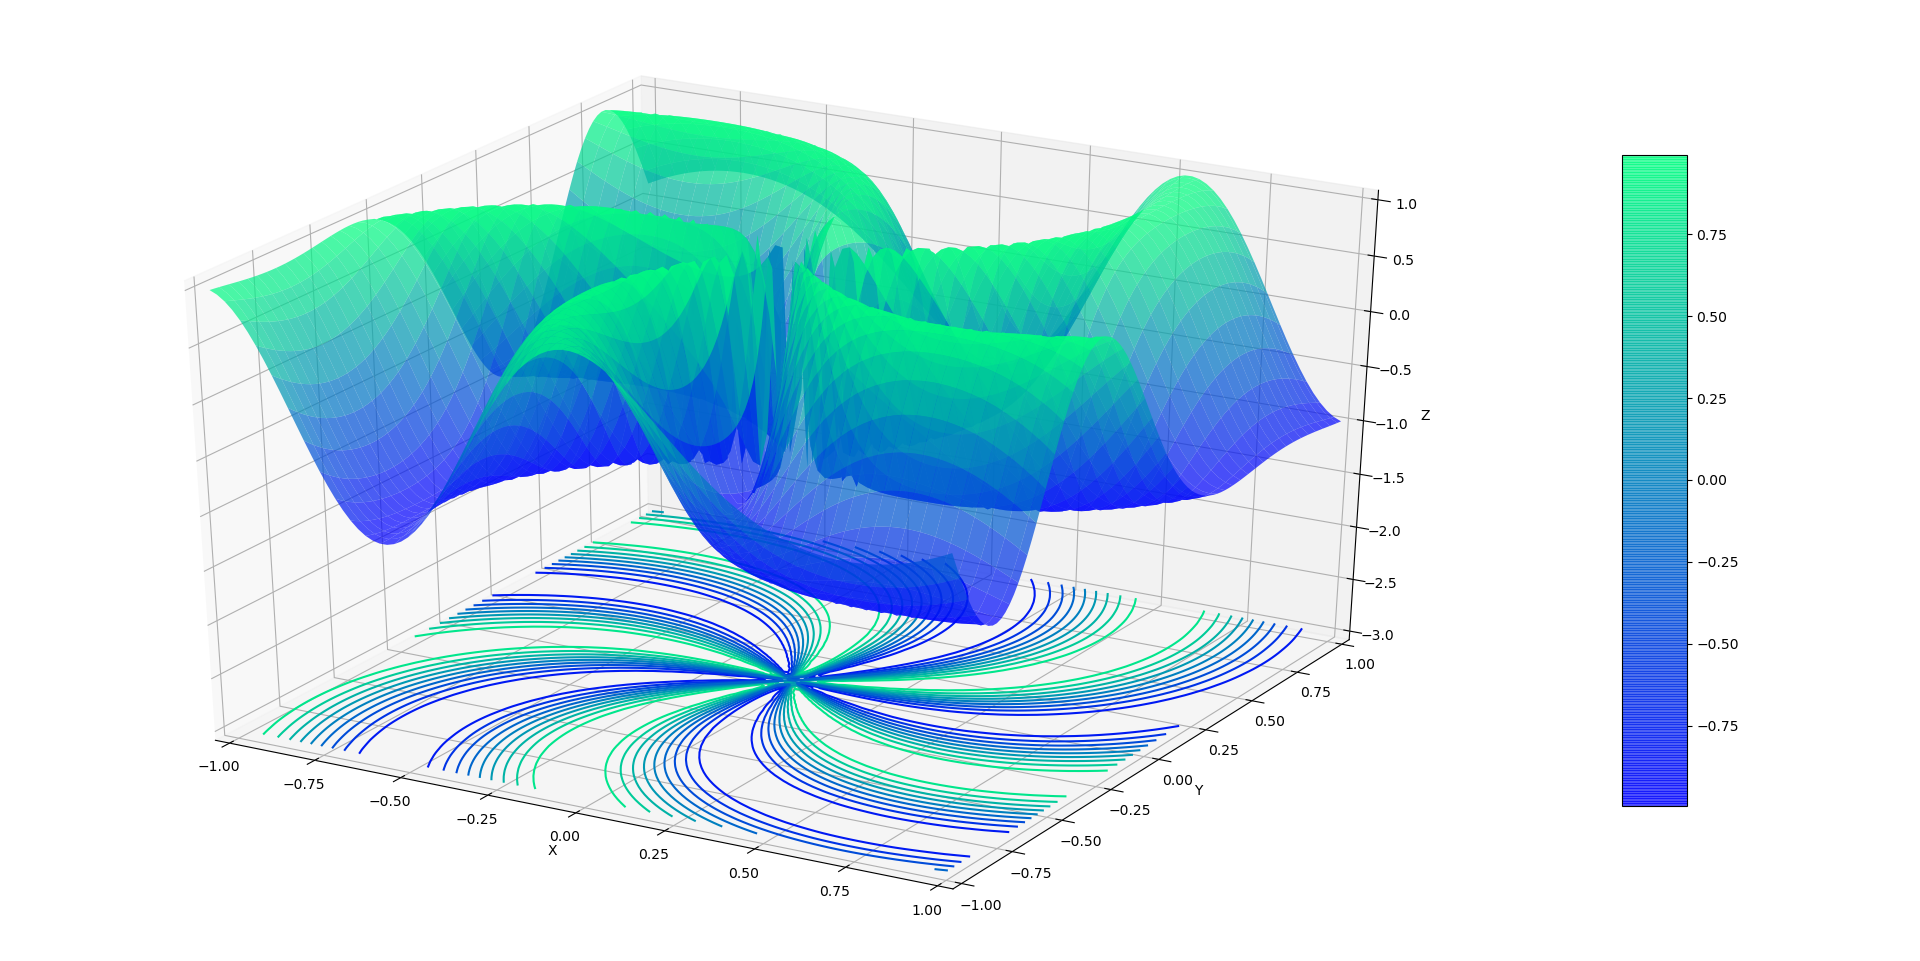
\includegraphics[width=0.8\textwidth]{1-2.png}
	\end{figure}
	
	\section*{Exercise 1.3 - Matplotlib: Data Input}
	Maximum = x:4.0 y:3.0 z:1.0
	\begin{figure}[!ht]
    \centering
	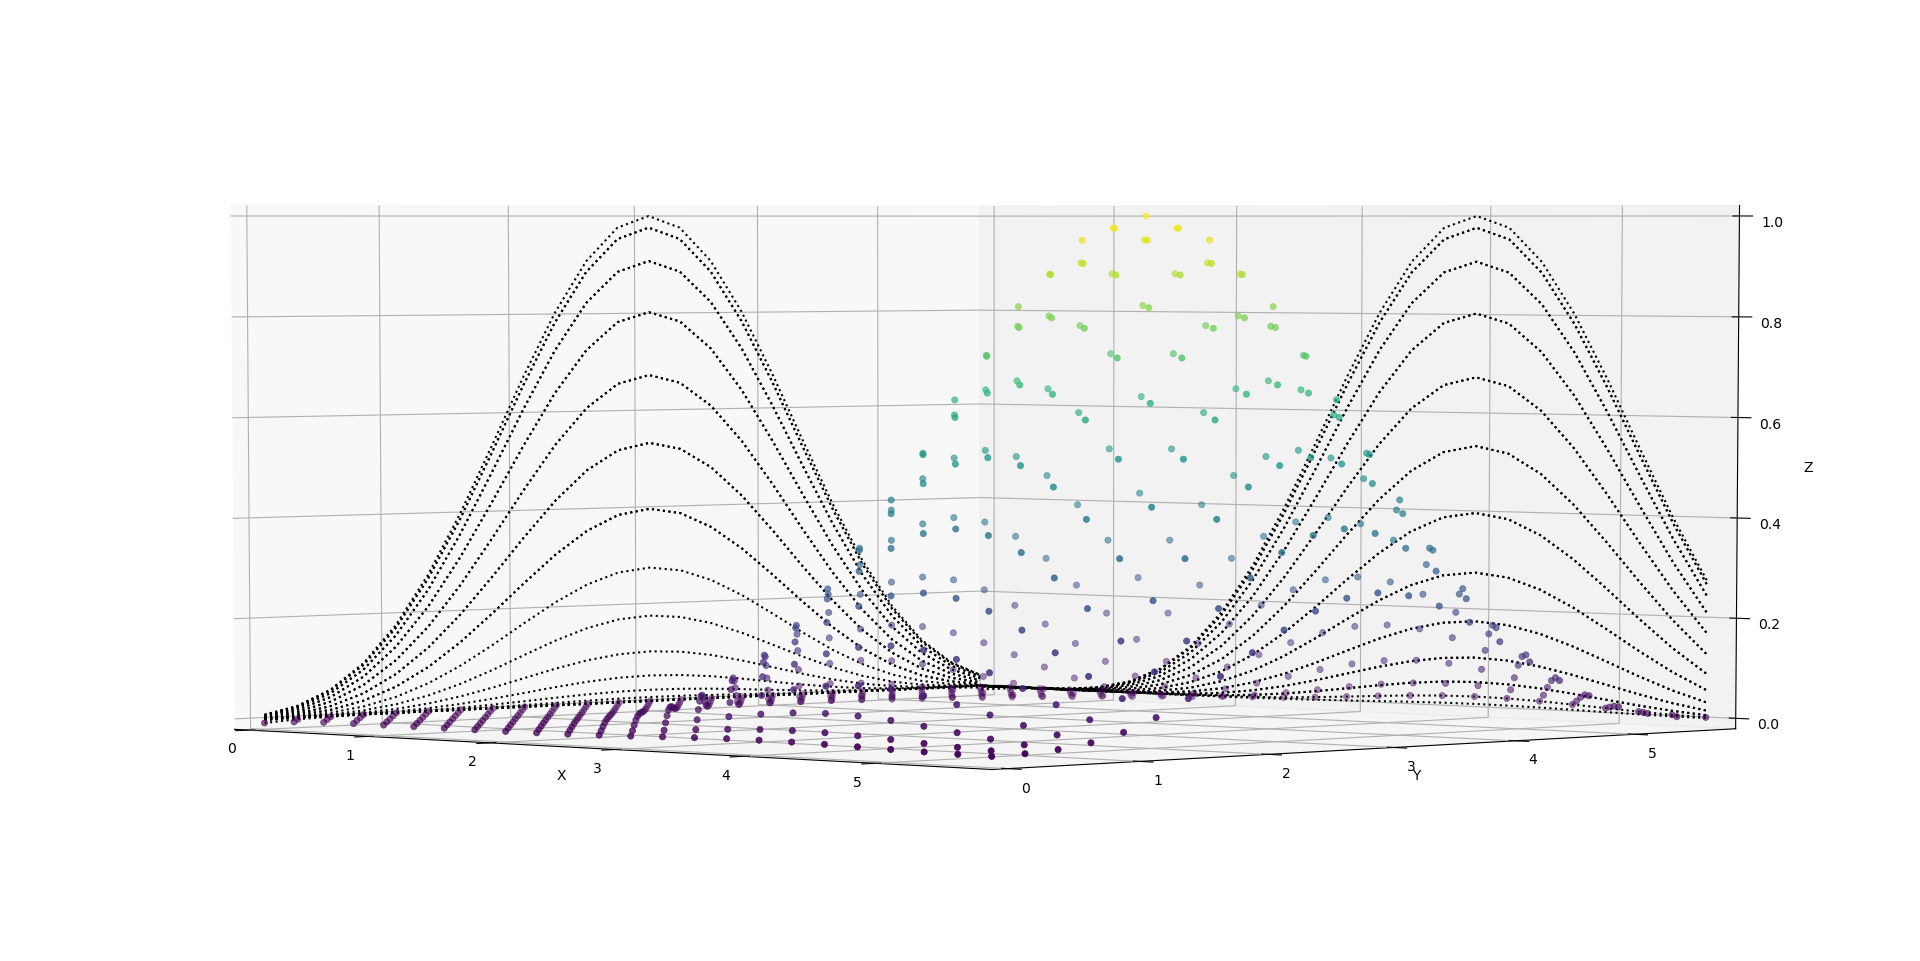
\includegraphics[width=0.8\textwidth]{1-3.png}
	\end{figure}
\end{document}
